\section{Digitální váha do hnízda}\label{sec:digitalni-vaha-do-hnizda}
Pro účely projektu bylo potřeba postavit digitální váhu.
Tato váha má být umístěna v každém hnízdě v kurníku, kde slepice snáší vejce, a jejím úkolem je přes \gls{usb} poskytovat aktuální data o tom, jakou hmotností je zatěžována podložka hnízda.

\subsection*{Popis algoritmu}
Po připojení napájení k Arduinu, se nejdříve nastaví a připojí sériová komunikace rychlostí 9600 baudů pomocí USB.
Následně je instancován objekt starající se o zprostředkování komunikace s převodníkem HX711~\cite{tenzosenzorahx711} a nastaví se jednotlivé piny dle fyzického zapojení převodníku.
Dále je nastaven kalibrační faktor, což je konstanta používaná knihovnou HX711.h při převodu dat získaných z převodníku na gramy, s nimiž program již nadále pracuje a následně je posílá po sériovém připojení.
Jako poslední krok v rámci přípravy programu je vynulování váhy pomocí metody tare(), která je jedna z metod HX711.h knihovny.
Jakmile program dokončí fázi příprav, vstoupí do nekonečného cyklu.
Tento cyklus pravidelně čte data přicházející po seriovém připojení.
V případě, kdy jsou přijata data, program počítá se třemi scénáři.
Buď je přijat znak "w", znak "t" nebo jakákoli jiná data.
V případě znaku "w" (od slova weight) program reaguje odesláním aktuální naměřené hodnoty váhy po sériovém připojení jako reakce na příkaz.
Přijatý znak "t" znamená tare neboli vynulovat váhu.
Na základě toho se programu řekne, že aktuální hodnotu, kterou získal ze senzoru, má brát jako hmotnost 0 g.


\subsection*{Konstrukce váhy}
Jako řídící jednotka váhy je použito Arduino Nano~\cite{ArduinoNano}, jež je zodpovědné za komunikaci s počítačem pomocí sériového připojení a načítání dat o hmotnosti z AD převodníku HX711 přes, který je Arduino připojeno k tenzometrickému~\cite{tenzosenzorahx711} senzoru.
Hmotnost je měřena tenzometrickým senzorem se jmenovitým zatížením 20 kg.
Toto zapojení je nutné vzhledem ke konstrukci a vlastnostem senzoru.
Tenzometrické senzory jsou analogové a jejich výstupem jsou velmi malé změny v napětí v rozmězí 0.15 až 1 mV.
Tyto signály jsou navíc hodně slabé, proto je nutné použít konkrétně převodník HX711, který signál zesílí a zajistí větší rozlišení díky vysoké citlivosti.
Složitější zapojení není jedinou nevýhodou.
Značnou nevýhodu představuje také fakt, že už vlivem zatížení se profil senzoru mírně deformuje a na základě toho narůstá chyba měření v průběhu času.
Tento problém se dá snadno řešit pravidelným nulováním v případech, kdy zrovna senzor zatížen není.
Na konstrukci váhy je velmi zajímavý tvar a důvody samotné železné konstrukce.
Protože má být váha instalována do již existujícího hnízda a slepice bude vlastně sedět rovnou na váze.
Nakonec je jako platforma, na které slepice sedí, zvolena čtvercová miska o rozměrech odpovídající s rezervou rozměrům celého hnízda.
Nemohla by to být například pouze rovná deska, protože slepice potřebuje pro pohodlné sezení podestýlku, kterou tvoří seno a v případě řešení s deskou by se seno dostalo mezi stěny hnízda a desku a váha by se tak nemohla volně pohybovat a zasekávala by se.
Takto v misce je mnohem menší šance, že bude nějak větší množství sena vytlačeno a bude přidírat váhu (obrázek~\ref{fig:instalace_vaha_hnizdo}~a~\ref{fig:vaha_prototyp2}).

\begin{figure}[H]
    \centering
    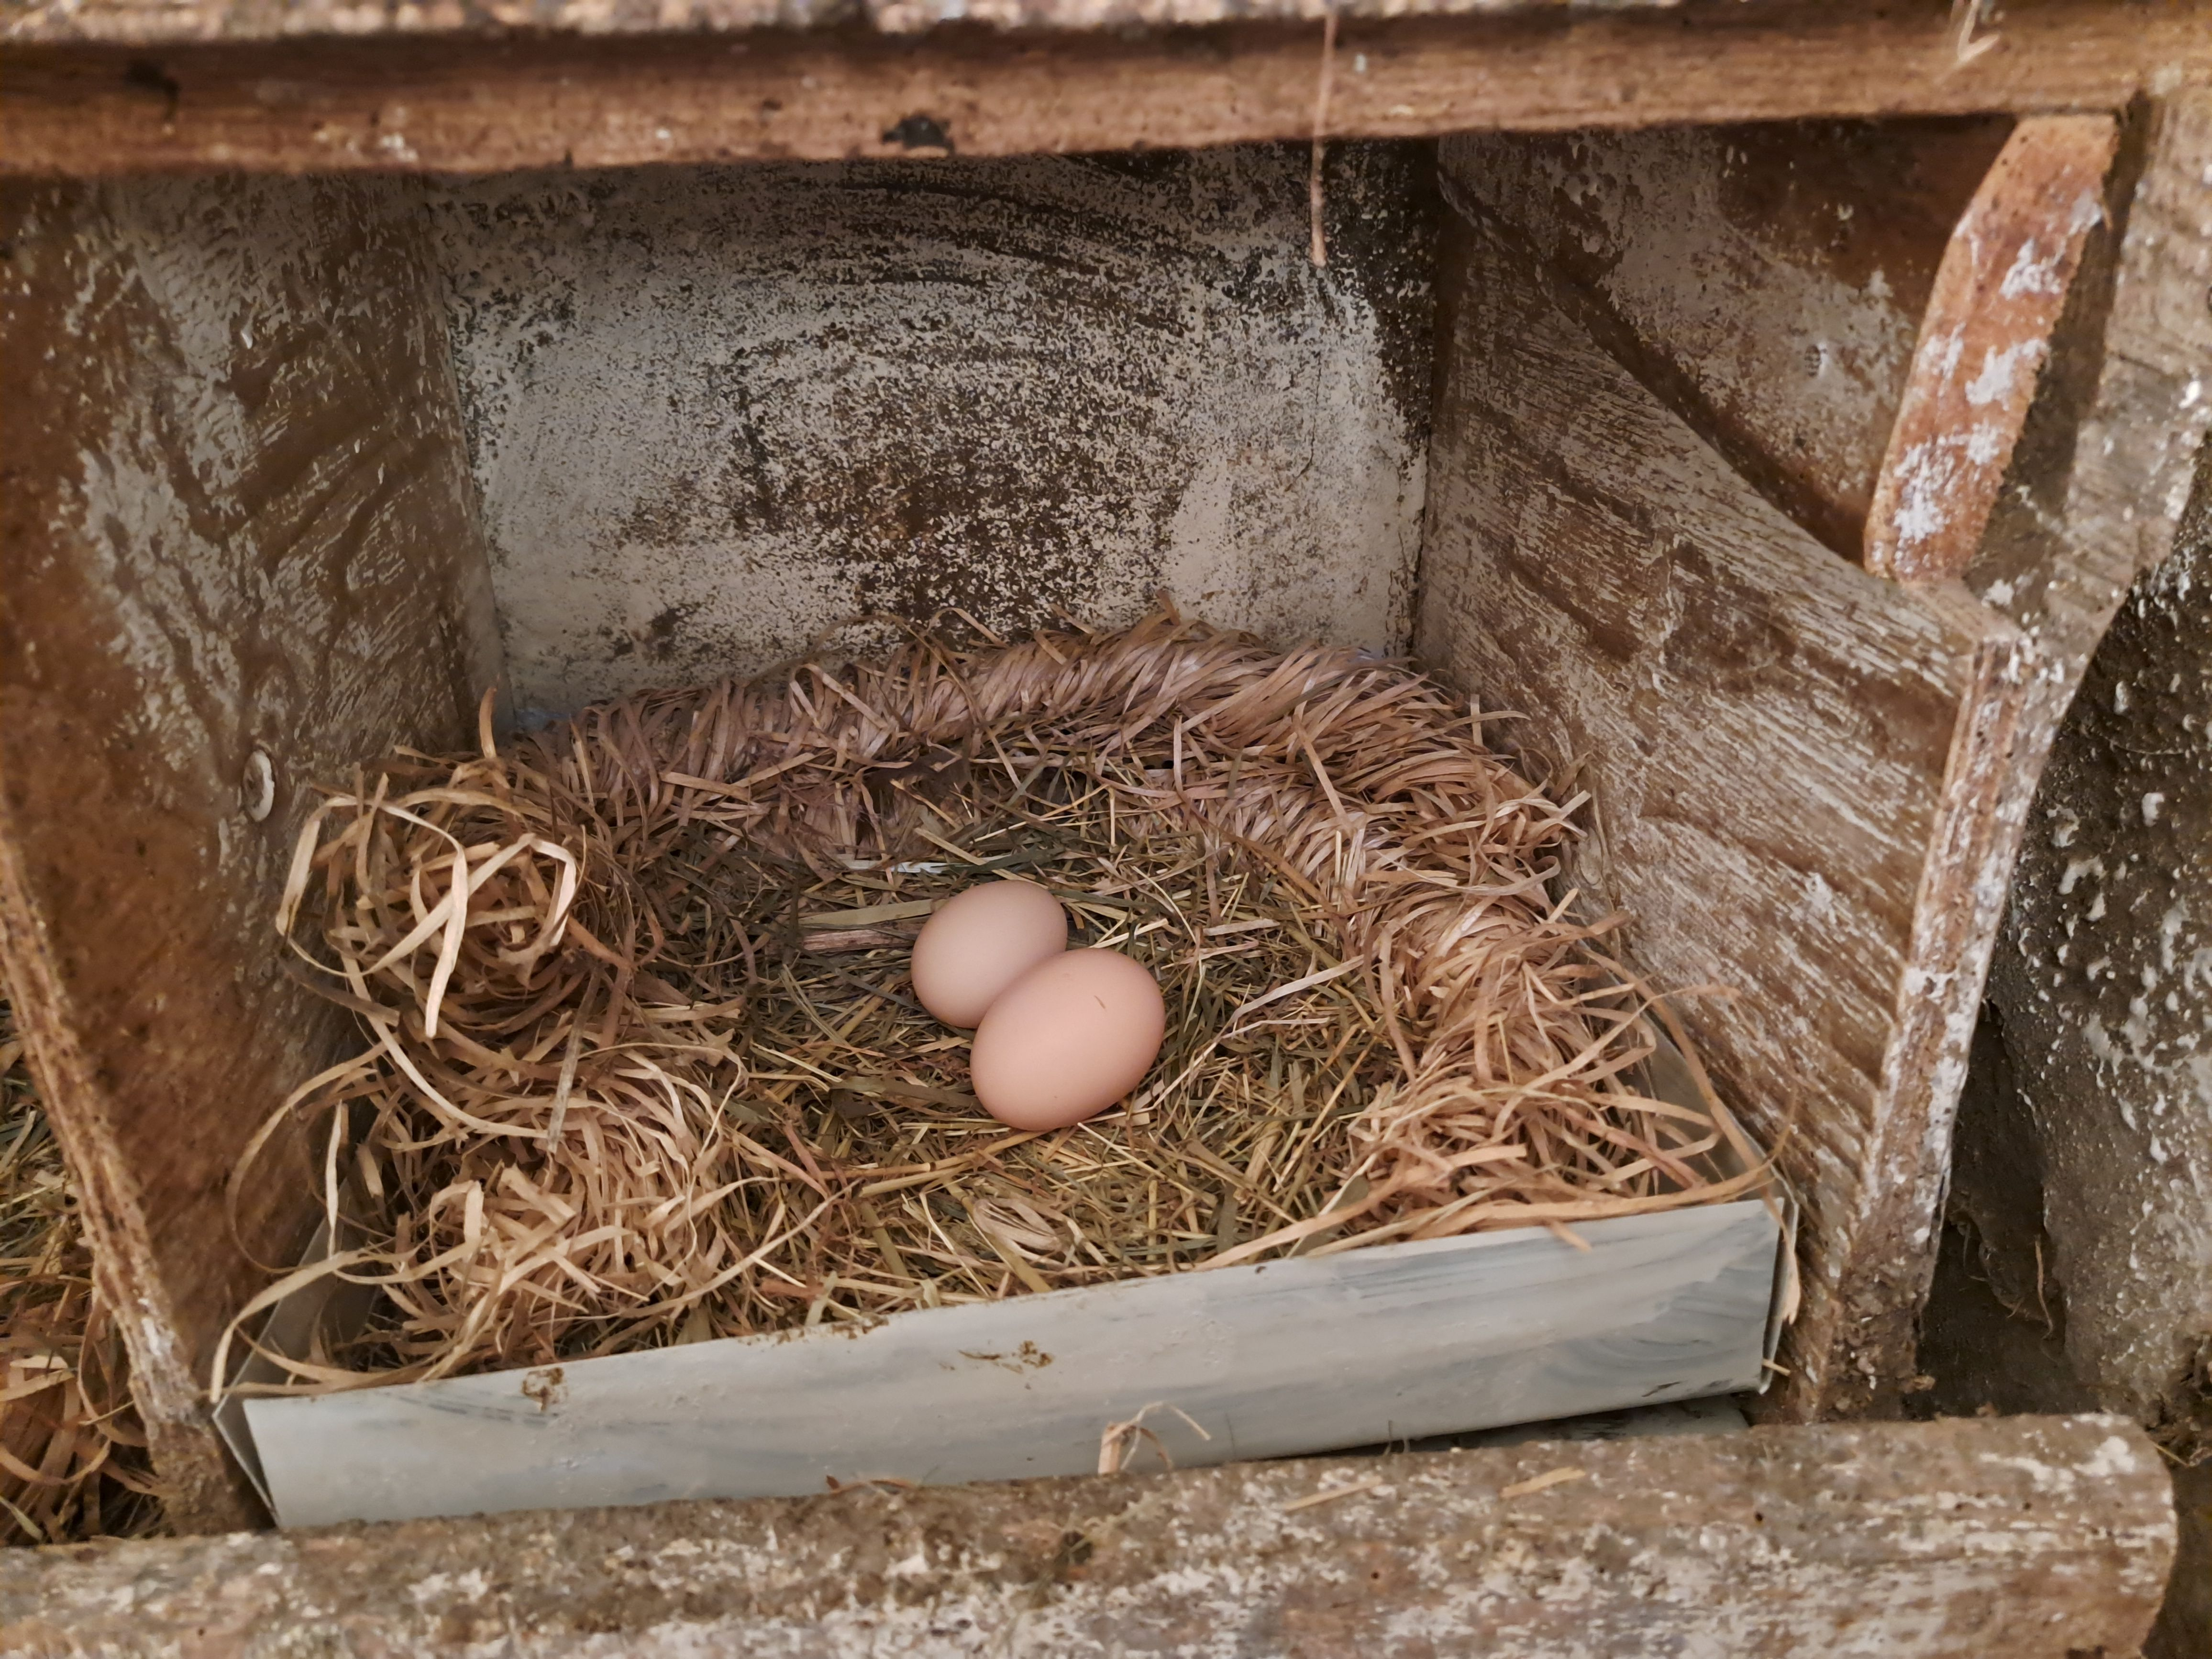
\includegraphics[width=0.8\textwidth]{img/instalace_vaha_hnizdo}
    \captionAuthorSource{První prototyp váhy instalovaný v hnízdě}
    \label{fig:instalace_vaha_hnizdo}
\end{figure}

\begin{figure}[H]
    \centering
    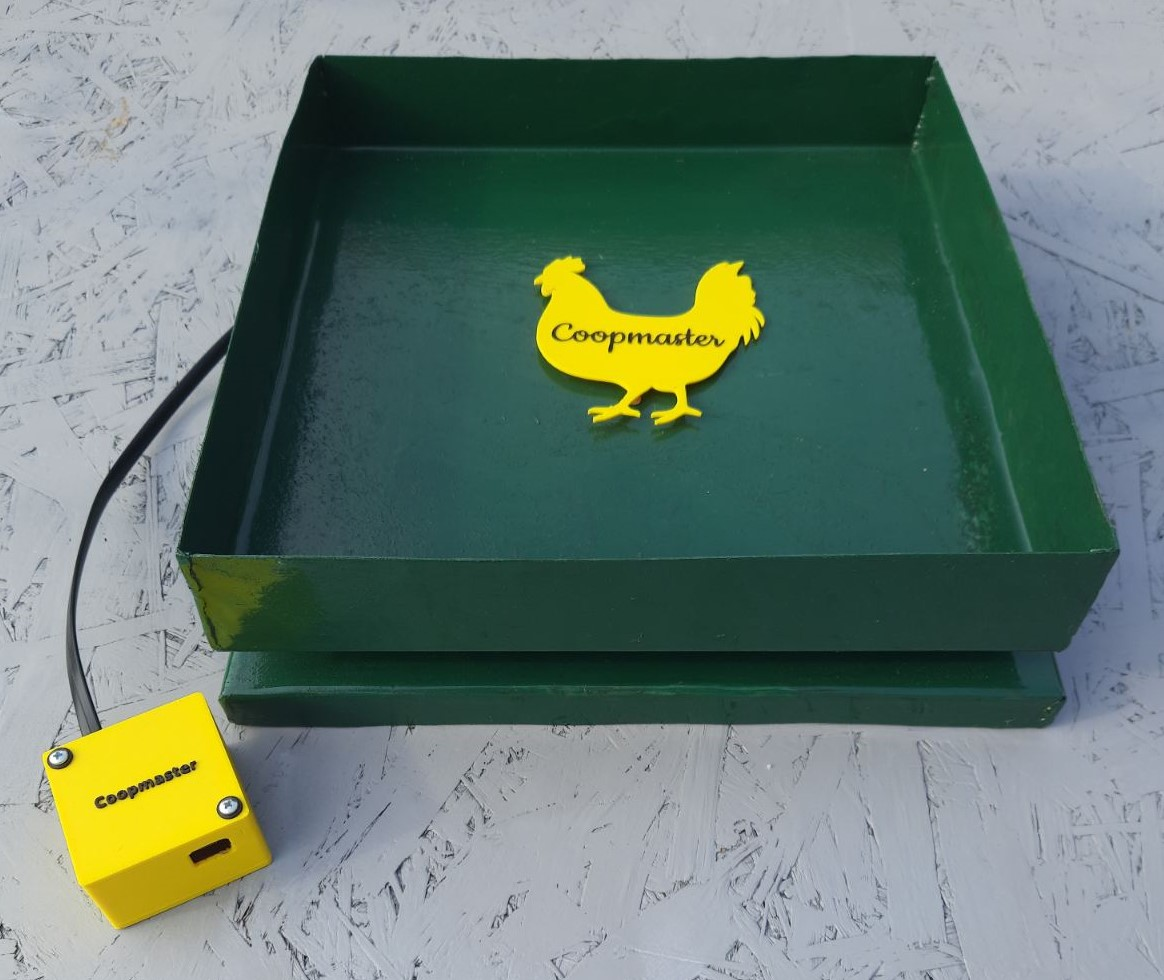
\includegraphics[width=0.8\textwidth]{img/vaha_prototyp2}
    \captionAuthorSource{Druhý prototyp váhy s logem}
    \label{fig:vaha_prototyp2}
\end{figure}

\subsection*{Kalibrace}
Po fyzickém sestavení váhy je třeba provést kalibraci.
Kalibrace používaných senzorů je nutná, protože se díky ní eliminují rozdíly mezi senzory, překryjí se nedostatky konstukce váhy a zajistí přesnost a korektnost měření pro konkrétní senzor.
To znamená najít vhodnou hodnotu kalibračního faktoru, která se již za běhu váhy nebude měnit.
Doporučená metoda, jak provádět kalibraci, je vzít si předmět, o němž víme přesně jeho hmotnost a ten použít jako vzorové závaží, na které chceme váhu kalibrovat.
Konkrétně u mnou použitého senzoru do 20 kg je dobré volit závaží v řádech minimálně několika kil.
Já jsem doma použil 5 balíčků polohrubé mouky.
Hmotnost balení jsem si ověřil přesnou kuchyňskou váhou.
Následujícím krokem je nalezení odpovídající hodnoty kalibračního faktoru pro náš senzor.
Položil jsem známé závaží na váhu a zvyšováním nebo snižováním kalibračního faktoru, jsem sedoval, jestli se návratová hodnota na vystupu, při aktuálním faktoru přibližuje nebo vzdaluje k hodnotě hmotnosti závaží na váze.

\subsection*{Hardware}
\begin{itemize}
    \item Arduino Nano v3.0
    \item AD převodník HX711
    \item Tenzometrický senzor se jmenovitým zatížením do 20 kg
    \item Železná konstrukce váhy
\end{itemize}

\subsection*{Arduino knihovny}
\begin{itemize}
    \item Arduino.h - základní Arduino knihovna
    \item HX711.h - pro usnadnění komunikace s AD převodníkem HX711
\end{itemize}

%- vysvětlit přijimane commandy w - dej vahu a t - tare
%zastrcim arduino do elektriky
%rozběhne se loop
%z pinů xy čteme hodnoty
%knihovna zpracovava hodnoty odporu
%knihovna řeší vynulování váhy
%vysvětlit kalibraci
%najít a popsat kalibrační program a vysvětlit k čemu je potřeba
%loop čeka a kontroluje serialovy vstup zda neni pismenko w nebo t
%popis loopu

%je tam převodník pro převod analogu na digital
%odecita odpor
%na konci toho je tenzometrikej můstek
%specifikace senzoru
%plusy a mínusy senzoru deformace, vysvětlit princip

%tenzometricky sezor podobne jako u vcel
%hezky popsano v praci
%uvaha o tom co vybrat zavesna vaha nebo tlacna vaha
%problemy pri implementaci
%problémy s konstrukcí a nekvalitními součástkami
%senzory se deformují a tím vzniká chyba v měření
%chyby vznikají díky analogu i chybami / odpory v elektrickém
%vedení (pevné / pájene spoje vs odnímatelné konektrory)

%knihovny arduina
%defaultní Arduino.h
%HX711.h: knihovna pro komunikaci s module AD Převodníku 24-bit 2 kanály HX711